\documentclass[
  a4paper,
  abstract=true,
  twoside,
  listof=totoc,
  numbers=noenddot,
  bibliography=totoc,
  BCOR1.5cm,
  headsepline,
  DIV12,
  appendixprefix,
  final
] {scrreprt}

% You should select either american or british instead of english here:
\usepackage[american,ngerman]{babel}
% \usepackage{cmap}
% \usepackage[utf8]{inputenc}
% \usepackage[T1]{fontenc}
\usepackage{fontspec}

\usepackage[pdftex,
citebordercolor={0.75 0.75 1},
filebordercolor={0.75 0.75 1},
linkbordercolor={0.75 0.75 1},
% pagebordercolor={0.75 0.75 1},
urlbordercolor={0.75 0.75 1},
pdfborder={0.75 0.75 1},plainpages=false,pdfpagelabels=true]{hyperref}
\hypersetup{%
  pdftitle={Simulation of a Scheduling Algorithm for DAG-based Task Models},
  pdfauthor={Maksym Planeta},
  pdfkeywords={foo, bar},
}

\usepackage[backend=biber,style=alphabetic,alldates=long]{biblatex}

\usepackage{varioref}           % nice refs
\usepackage{csquotes}
\usepackage{graphicx}           % graphics
\usepackage{caption}            % manipulate fugures
\usepackage{subcaption}         % allow for subfigures
\usepackage{listings}           % nice source code listings
\usepackage{color}
\usepackage{booktabs}           % nice tables
\usepackage{microtype}          % better looking text borders
\usepackage{units}              % unified way of setting values with units
\usepackage{array}
\usepackage{fancybox}           % provide nice boxes
\usepackage{units}              % unified way of setting values with units
\usepackage{fancyvrb}           % algorithm-boxes
\usepackage{pdfpages}
\usepackage{hyphenat}
\usepackage{todonotes}
\usepackage{xspace}
\usepackage{setspace}
\usepackage{tikz}
\usepackage{amsmath}
\usepackage{amssymb}
\usepackage{mathtools}
\usepackage{subcaption}

\ifdefined\pdffontattr% \ifdefined is part of the e-TeX extension, which is part of any modern LaTeX compiler. 
    \immediate\pdfobj stream file {umsa.cmap}
    {\usefont{U}{msa}{m}{n}\pdffontattr\font{/ToUnicode \the\pdflastobj\space 0 R}}
    \immediate\pdfobj stream file {umsb.cmap}
    {\usefont{U}{msb}{m}{n}\pdffontattr\font{/ToUnicode \the\pdflastobj\space 0 R}}
\fi

% use this one last
% (redefines some macros for compatibility with KOMAScript)
\usepackage{scrhack}

\addbibresource{/home/desertfox/research/refs.bib} 
% \addbibresource{own.bib}
\input{preamble/color.tex}
 
% Biblatex Style
\setcounter{secnumdepth}{3}     % limit enumeration depth
\setcounter{tocdepth}{1}        % limit TOC depth

% Listing Style

\lstset{ %
  frame=shadowbox,
  rulesepcolor=\color{blue},
  backgroundcolor=\color{white},   % choose the background color; you must add \usepackage{color} or \usepackage{xcolor}
%  basicstyle=\footnotesize,        % the size of the fonts that are used for the code
  breakatwhitespace=false,         % sets if automatic breaks should only happen at whitespace
  breaklines=true,                 % sets automatic line breaking
  captionpos=b,                    % sets the caption-position to bottom
  commentstyle=\color{mygreen},    % comment style
  deletekeywords={...},            % if you want to delete keywords from the given language
  escapeinside={\%*}{*)},          % if you want to add LaTeX within your code
  extendedchars=true,              % lets you use non-ASCII characters; for 8-bits encodings only, does not work with UTF-8
  frame=single,                    % adds a frame around the code
  keepspaces=true,                 % keeps spaces in text, useful for keeping indentation of code (possibly needs columns=flexible)
  keywordstyle=\color{blue},       % keyword style
  language=C,                 % the language of the code
 % morekeywords={*,...},            % if you want to add more keywords to the set
  numbers=left,                    % where to put the line-numbers; possible values are (none, left, right)
  numbersep=7pt,                   % how far the line-numbers are from the code
  numberstyle=\tiny\color{mygray}, % the style that is used for the line-numbers
  rulecolor=\color{black},         % if not set, the frame-color may be changed on line-breaks within not-black text (e.g. comments (green here))
  showspaces=false,                % show spaces everywhere adding particular underscores; it overrides 'showstringspaces'
  showstringspaces=false,          % underline spaces within strings only
  showtabs=false,                  % show tabs within strings adding particular underscores
  stepnumber=1,                    % the step between two line-numbers. If it's 1, each line will be numbered
  stringstyle=\color{mymauve},     % string literal style
  tabsize=2,                       % sets default tabsize to 2 spaces
  title=\lstname                   % show the filename of files included with \lstinputlisting; also try caption instead of title
}

% Typesetting options
\tolerance 2414
\hbadness 2414
\emergencystretch 1.5em
\hfuzz 0.3pt
\widowpenalty=10000     % Hurenkinder
\clubpenalty=10000      % Schusterjungen
\vfuzz \hfuzz
\raggedbottom

% use nice footnote indentation
\deffootnote[1em]{1em}{1em}{\textsuperscript{\thefootnotemark}\,}

\usetikzlibrary{
  shapes,
  arrows,
  fit,
  calc,
  positioning,
  graphs,
  trees,
  chains,
  calc,
  quotes
}


\tikzset{
  vertex/.style={circle,draw, fill=none, radius=100,minimum size = 15pt,inner sep=1pt},
  current/.style={circle,draw, fill=none, radius=100,minimum size = 15pt,inner sep=1pt},
  next/.style = {
    circle,draw,
    fill=yellow!30,
    radius=100,
    minimum size = 15pt,
    inner sep=1pt
  },
  future/.style = {
    circle,draw,
    fill=green!30,
    radius=100,
    minimum size = 15pt,
    inner sep=1pt
  },
  fogged/.style={circle,fill=none, radius=100,minimum size = 9pt,inner sep=1pt},
  label/.style={auto,draw=none,fill=none,color=black},
  slot/.style 2 args= {
    minimum width=0.8cm,
    fill=white,
    draw,
    below=0cm of #2,
    minimum height=#1cm / 2,
  },
}

 
% some common commands
\newcommand{\drops}{\texorpdfstring{\textsc{Drops}\xspace}{DROPS}}
\newcommand{\LLinux}{\texorpdfstring{L$\!^4$Linux}{L4Linux}}

\newcommand{\NOVA}{NOVA\xspace}
\newcommand{\QEMU}{QEMU\xspace}

\newcommand*\mean[1]{\overline{#1}}

% If you know when you will hand in your thesis, enter the date here.
\date{27. April 2015}
\newcommand{\printdate}{\@date}

\begin{document}

\pagenumbering{Roman}
\newtheorem{definition}{Definition}

 
\selectlanguage{american}

\begin{singlespace}

\subject{{\LARGE Master thesis}}

\title{Simulation of a Scheduling Algorithm for DAG-based Task Models}

\author{Maksym Planeta}

\publishers{Technische Universität Dresden\\
Fakultät Informatik\\
Institut für Systemarchitektur\\
Professur Betriebssysteme\\
\begin{minipage}{\textwidth}%\\
\vskip 6cm
 {\normalsize }\begin{tabular}{ll}
Betreuender Hochschullehrer: &
Prof. Dr. rer. nat. Hermann Härtig\tabularnewline
Betreuende Mitarbeiter: &
Dr.-Ing. Marcus Völp\tabularnewline
&Dr.-Ing. Michael Roitzsch\tabularnewline

\end{tabular} {\normalsize }\end{minipage}}

\maketitle
\end{singlespace}

\cleardoublepage

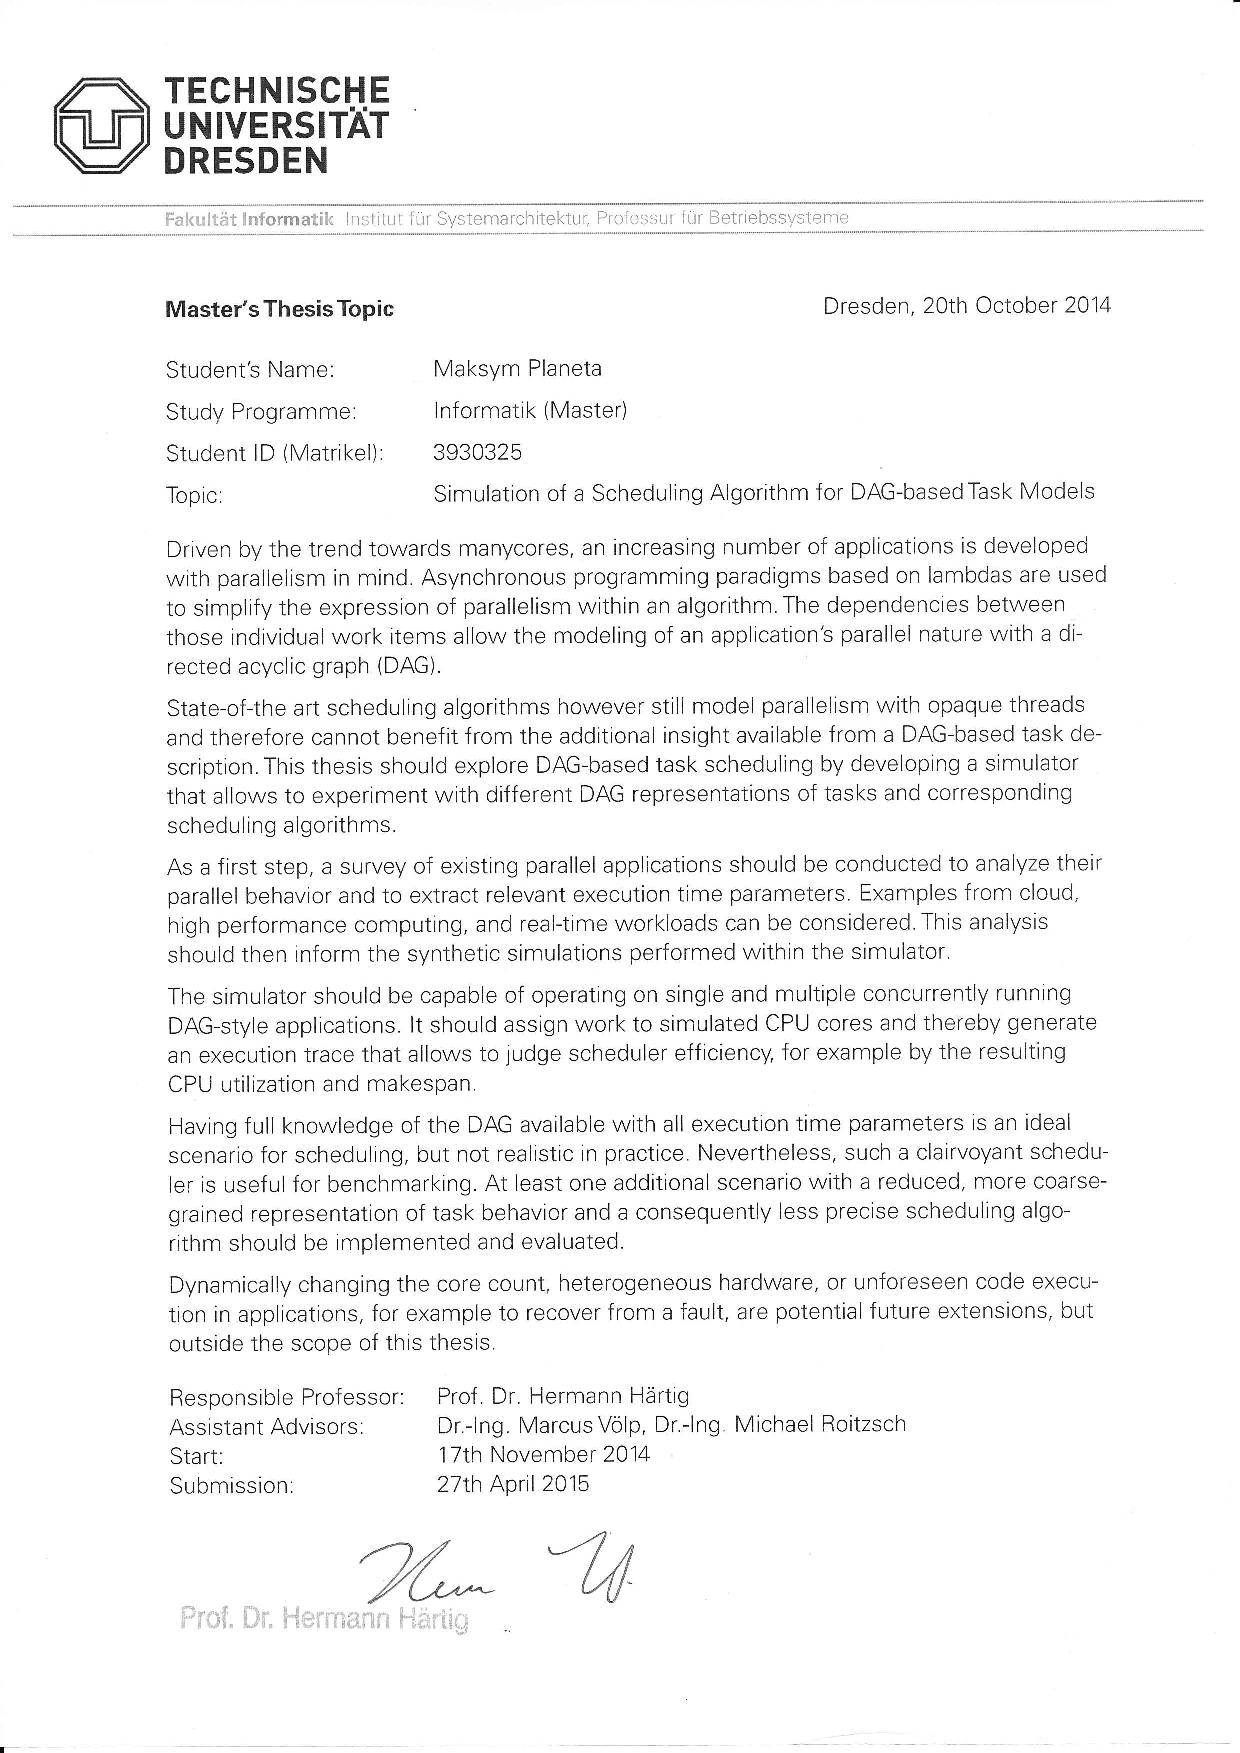
\includepdf{images/diplom-aufgabe.pdf}
\cleardoublepage

 
\selectlanguage{ngerman}

\section*{\vfill{} \thispagestyle{empty}
Erklärung}

Hiermit erkläre ich, dass ich diese Arbeit selbstständig erstellt
und keine anderen als die angegebenen Hilfsmittel benutzt habe.
\bigskip{}

\noindent Dresden, den \printdate % \printdate % if you defined date earlier
\vspace{2.5cm}

\noindent Maksym Planeta \cleardoublepage{}

% NOTE: if you selected british or american above, change that here too
\selectlanguage{american}

\begin{abstract}
\input{content/02_abstract.tex}
\end{abstract}

\cleardoublepage

\tableofcontents

\cleardoublepage

% remove this on final
\listoftodos
\cleardoublepage

\listoffigures
\cleardoublepage

\listoftables
\cleardoublepage

\pagenumbering{arabic}
\chapter{Introduction}
\label{sec:intro}

% Die Einleitung schreibt man zuletzt, wenn die Arbeit im Großen und
% Ganzen schon fertig ist. (Wenn man mit der Einleitung beginnt - ein
% häufiger Fehler - braucht man viel länger und wirft sie später doch
% wieder weg). Sie hat als wesentliche Aufgabe, den Kontext für die
% unterschiedlichen Klassen von Lesern herzustellen. Man muß hier die
% Leser für sich gewinnen. Das Problem, mit dem sich die Arbeit befaßt,
% sollte am Ende wenigsten in Grundzügen klar sein und dem Leser
% interessant erscheinen. Das Kapitel schließt mit einer Übersicht über
% den Rest der Arbeit. Meist braucht man mindestens 4 Seiten dafür, mehr
% als 10 Seiten liest keiner.


It is known that problem of scheduling parallel programs onto
multiprocessor computer in its general form is
NP-complete~\cite{Ullman1975}. There are know constrained models,
which allow to determine optimal schedule in polynomial
time~\cite{Hu1961, Coffman1972, Papadimitriou1979}.  But simplicity of
these models barely allows their utilization for scheduling of real
parallel applications.

Parallelization of an application requires extensive knowledge about
program structure. There exist a variety of methods to declare program
structure, that is convenient for the programmer, but also allows to
effectively schedule the application on multiprocessor system. Such
parallelization methods among others are fork-join pattern[links],
message-passing systems[links], map-reduce frameworks[links],
future-based parallelism[links], asynchronous lambda
approaches[links].

These methods differ in their API, in their granularity and
functionality. But all they have one common idea: order sequential
sections of the application in such temporal order that respects their
mutual dependencies. This process is called
\emph{scheduling}. Sequential sections represent parts of actual
execution trace of the program and have corresponding starting and
finish time. The same part of the application code can appear as
several sequential sections.

Dependencies between sequential sections represent transfers of data
that is calculated in precedent sections and used as an input by
subsequent ones. Relations between sequential sections can be modeled
as a graph, and thus all the dependencies go from past to future this
graph has no cycles. Thus, such model is called Directed Acyclic Graph
(DAG).

DAG is a common and well-studied way to represent the execution of
parallel application \cite{zheng20131673,
  Blumofe:1996:ADD:237502.237574}.


\section{Motivation}

\section{Document Structure}



% Referencing other chapters: \ref{sec:state} \ref{sec:design}
% \ref{sec:implementation} \ref{sec:evaluation} \ref{sec:futurework}
% \ref{sec:conclusion}

% \begin{table}[htp]
%   \centering
%   \begin{tabular}{lrr}
%     \textbf{Name} & \textbf{Y} & \textbf{Z} \\
%     \hline
%     \textit{Foo} & 20,614 & \unit[23]{\%} \\
%     \textit{Bar} & 9,914 & \unit[11]{\%} \\
%     \textit{Foo + Bar} & 30,528 & \unit[34]{\%} \\
%     \hline
%     \textit{total} & 88,215 & \unit[100]{\%} \\

%   \end{tabular}
%   \caption[Some interesting numbers]{Various very important looking numbers and sums.}
%   \label{tab:numbers}
% \end{table}

% More text referencing Table~\ref{tab:numbers}.

% \section{Another Section}

% \begin{figure}[tbp]
%   \centering
%   \includegraphics[width=0.8\textwidth]{images/squirrel}
%   \caption[Short description]{A long description of this squirrel figure.
%   Image taken from
%   \url{http://commons.wikimedia.org/wiki/File:Sciurus-vulgaris_hernandeangelis_stockholm_2008-06-04.jpg}}
%   \label{fig:squirrel}
% \end{figure}

% Citing \cite{bellard2005qfa} other documents \cite{bellard2005qfa, boileau06}
% and Figure~\ref{fig:squirrel}.

% Something with umlauts and a year/month date:
% \cite{becher04:_feurig_hacken_mit_firew}.

% And some online resources: \cite{green04}, \cite{patent:4819234}

% \section{Yet Another Section}

% \todo{add content}

% \begin{figure}[tbp]
%  \missingfigure{Come up with a mindblowing figure.}
%  \caption{A mindblowing figure}
%  \label{fig:todo}
% \end{figure}

% \section{Test commands}

% \drops \LLinux \NOVA \QEMU
% \texttt{memcpy}
% A sentence about BASIC. And a correctly formatted one about ECC\@.

\cleardoublepage

%%% Local Variables:
%%% TeX-master: "diplom"
%%% End:

\chapter{Technical Background}
\label{sec:state}

% Hier werden zwei wesentliche Aufgaben erledigt:

% 1. Der Leser muß alles beigebracht bekommen, was er zum Verständnis
% der späteren Kapitel braucht. Insbesondere sind in unserem Fach die
% Systemvoraussetzungen zu klären, die man später benutzt. Zulässig ist
% auch, daß man hier auf Tutorials oder Ähnliches verweist, die hier auf
% dem Netz zugänglich sind.

% 2. Es muß klar werden, was anderswo zu diesem Problem gearbeitet
% wird. Insbesondere sollen natürlich die Lücken der anderen klar
% werden. Warum ist die eigene Arbeit, der eigene Ansatz wichtig, um
% hier den Stand der Technik weiterzubringen? Dieses Kapitel wird von
% vielen Lesern übergangen (nicht aber vom Gutachter ;-), auch später
% bei Veröffentlichungen ist "Related Work" eine wichtige Sache.

% Viele Leser stellen dann später fest, daß sie einige der Grundlagen
% doch brauchen und blättern zurück. Deshalb ist es gut,
% Rückwärtsverweise in späteren Kapiteln zu haben, und zwar so, daß man
% die Abschnitte, auf die verwiesen wird, auch für sich lesen
% kann. Diese Kapitel kann relativ lang werden, je größer der Kontext
% der Arbeit, desto länger. Es lohnt sich auch! Den Text kann man unter
% Umständen wiederverwenden, indem man ihn als "Tutorial" zu einem
% Gebiet auch dem Netz zugänglich macht.

% Dadurch gewinnt man manchmal wertvolle Hinweise von Kollegen. Dieses
% Kapitel wird in der Regel zuerst geschrieben und ist das Einfachste
% (oder das Schwerste weil erste).

This thesis presents a new algorithm for scheduling DAG-based parallel
applications. The algorithm attempts to fill the niche between two
classes of algorithms for parallel applications. Algorithms from the
first class are aware of the DAG structure of the application and try
to use this knowledge to optimize the resulting schedule. We call this
class of algorithms \emph{DAG-algorithms}. Representatives of another class are
unaware of DAG structure of the application and make scheduling
decision without any advance knowledge of future program behavior. We
call this class of algorithms \emph{ready queue algorithms}.

In following section these two algorithms and their corresponding
system models will be described in detail. Additionally there will be
given deeper classification of DAG aware algorithms. Several important
representatives of each class will be outlined.

\section{Ready queue algorithms}

First, we will start with dynamic algorithms. The reason for that is
that they are simpler, they have simpler system model and can be
easily ported to the environment where dag-algorithms act.We call
algorithm dynamic if it does not have any prospective knowledge of a
program structure. Hence, it does not have a phase before actual
program execution, where it can build up helper data structures.

Program is still assumed to consist of sequential pieces called
\emph{jobs}. Jobs have sequential dependencies between each other. If
two jobs have noncontradictory dependency sets, they can run in
parallel on different \emph{processing elements (PE)}.  Parallel
program can be modeled as a DAG where \emph{nodes} represent jobs and
edges represent \emph{edges}.

In ready queue algorithms DAG nodes appear for the scheduler only when
they become \emph{ready}, i.~e. all their dependencies get
satisfied. A job that is currently being executed on a PE is called
\emph{active}.

\begin{definition}
  If execution of a job $A$ depends on another job $B$, job $A$ is
  called a \emph{child} of a job $B$. And job $B$ is called a
  \emph{parent} of a job $A$.
\end{definition}

\subsection{Global queue algorithms}
\label{sec:global_queue}

The trivial system model assumes that there exist single globally
accessible list of nodes, which state is \emph{ready}. Such a list is
called \emph{ready list} \footnote{Also known as \emph{ready
    queue}.}. Whenever there is a PE with no active job, it tries to
grab one from a ready list.

Yet simple, but unrealistic, this model does not allow to achieve high
overall
performance. \citeauthor{anderson1989performance}~\cite{anderson1989performance}
have \todo{Which number to use? Singular for a ``paper''? Plural for
  the ``authors''? Now it is a mess.} shown that contention for the
system bus can drastically decreases both system latency and
throughput. Various researches have shown the influence of the data
locality on the number of CPU cache
misses~\cite{Spoonhower:2009:BNP:1583991.1584019,Herlihy:2014:WFC:2555243.2555257,Squillante1993}
and page faults~\cite{Blumofe:1996:ADD:237502.237574}. This increases
shared memory bus traffic and contention and bring significant
performance penalty. \cite{Squillante1993} has shown that if child
jobs tend to stay on the same CPU as parents, performance penalty
grows slower with increased number of PEs.

\subsection{Work stealing algorithms}
\label{sec:work_stealing}

There exist two major dynamic scheduling paradigms where jobs tend to
stay where parents have been run: \emph{work stealing} and \emph{work
  sharing}~\cite{Blumofe:1999:SMC:324133.324234}. To enforce this
principle each PE maintains its own \emph{local ready list}. In work
stealing paradigm, PEs take or \emph{steal} jobs from ready lists of
other PEs. And in work sharing ones, PEs pass or \emph{share} jobs from
their ready list to the ready lists of other PEs.

Principles of work sharing algorithms are similar to work stealing
ones, but the latter ensure less communication
overhead~\cite{Blumofe:1999:SMC:324133.324234}, thus we will describe
only work stealing paradigm in detail.

Work stealing algorithms are subject of extensive
research~\cite{Spoonhower:2009:BNP:1583991.1584019,Blumofe:1999:SMC:324133.324234,Acar:2000:DLW:341800.341801,Arora:1998:TSM:277651.277678},
but also have number of practical
implementations~\cite{Halstead:1984:IML:800055.802017,Blumofe:1995:CEM:209937.209958}.
Execution environment where typical work stealing algorithm acts has
following structure. There exist a set of PEs that can compute
parallel tasks independently. Each PE has its own ready list. When a
PE finishes the job, some of the children of this job can become
ready. If it happens, than these children are added to the local
\emph{ready queue} of the PE.

Each PE is capable to communicate with any other PE. This
communication could involve data transfers required to complete the
job, but also PEs are capable to communicate to exchange the jobs in
their working queues. The process of exchanging jobs among ready
queues is the essence of scheduling for dynamic scheduling algorithms.

A PE attempts to steal a job only when its own queue becomes
empty\footnote{Such a work stealing schedulers are called
  \emph{parsimonious}~\cite{Spoonhower:2009:BNP:1583991.1584019}.}.

\todo{Write more here}

\subsection{Delay scheduling}
\label{sec:delay}

\cite{zaharia2010delay} propose an interesting ready queue algorithm for clusters

\section{DAG-algorithms}
\label{sec:dag_algs}

If a program structure is known beforehand, it is possible to develop
more complicated algorithms. Number of examples are know in the
research~\cite{wu1990hypertool,bittencourt2010dag,wu2000mcp,adam1974,kwok1999static,zheng20131673,Topcuoglu2002}. All
these algorithms differ in the approach proposed but as well in the
model where the algorithm operates. An example of algorithm types
classification is given in~\cite{kwok1999static}.

Further in this section we will give an overview of popular algorithms
and system models. Although we separate scheduling heuristics in
several subsections it is important to mention that they often can be
combined in the same algorithm to improve overall performance. Good
example of such combination is a combination of clustering heuristic
(see Section~\ref{sec:clustering}) and task duplication heuristic (see
Section~\ref{sec:duplication}). An example of such combination is LCTD
algorithm~\cite{chen1993performance}. \todo{This paper is not
  available online. Is legit to cite it? Too reference and description from Kwok.}

\subsection{System model}
\label{sec:model}

Besides structure of the DAG itself important characteristic of the
system model of the algorithm is the information that is known about
the jobs and job communication. In simplest case, we can assume that
anything, except job precedence constraints is irrelevant. In this
situation jobs are assumed to have \emph{unit} computational costs
(i.~e. all computational costs are equal for all the
jobs)~\cite{Hu1961,adam1974}. If computation costs are under
consideration, than node weight can have arbitrary value. And this
value represents time required to complete a job on a PE. If
communication is irrelevant edge weight is either uniform for all the
edges or zero. UET-UCT (unit estimated time-unit communication time)
is a typical model in research area~\cite{finta1996scheduling,
  andronikos2000optimal}, which assumes both computation and
communication costs have unit weight.

The popular model which operates with arbitrary node and edge weights
is called \emph{macro dataflow}
model~\cite{yang1992pyrros,wu1990hypertool}.  Without explicitly
naming it, this model can also be found in numerous other
papers~\cite{adam1974, kwok1999static, sakellariou2004low}\todo{Should
  I mention all the papers having this property?}. Macro dafaflow
model works as follows. The execution runs respecting the dependencies
between the jobs in a DAG. Each job runs exclusively on certain PE for
the time, which depends on the computational\todo{computational or
  computation?}  costs of the job. These costs can have arbitrary
finite value. Before a job starts it should receive data from its
parent. Time required to accomplish this operation depends on the
communication costs of the job and also can have arbitrary finite
value. When two a parent and a child run on the same PE communication
between them takes no time.

Macro dataflow model yet simple, but often precise enough to
approximate execution of parallel program and multiprocessor system
running it. The assumption of zero communication costs within the same
PE is realistic because throughput of the network is much lower than
the throughput of physical ram. Moreover, it is often the case, that
data should not be moved, if job consuming the data resides on the
same PE as the job generated the data.

Modern systems are often heterogeneous. This requires algorithms to
cope with heterogeneous systems as well. Computing system can have to
kinds of heterogeneity, which can also be combined in the same system:
heterogeneity of PEs~\cite{grajcar1999genetic, Topcuoglu2002,
  arabnejad2014list} and heterogeneity of
communication~\cite{arabnejad2014list,
  bittencourt2010dag}. Heterogeneity of PEs means that instead of
single node weight, each job has defined table of execution times for
each PE that exist in the system. Different communication channels
between PEs imply different time requirements for a data transfers,
which happen to fulfill job's dependency requirements.

System topology also can bring significant complication for an
algorithm. Being fully connected graph (\emph{clique}) in the simplest
case, connections between PEs can form arbitrary structures. Clique,
Hypercube, Fat Tree are popular topologies. But sometimes combinations
of famous structures or irregular structures should be handled. The
reasons for such a diversity are expenses, throughput, latency and
reliability, which vary for different topologies\todo{No need for
  refs. This is general knowledge. Right?}. Irregular structures occur
when ownership of a network is decentralized\todo{refs}.

Depending on existence of the restriction of the DAG algorithms are
divided in \emph{arbitrary graph structure} algorithms and
\emph{restricted graph structure}
algorithms. \citeauthor{Hu1961}~\cite{Hu1961} \todo{What is the better
  form to make such quotations?} requires the program to have a
tree-structure and the jobs to have unit computational
costs. \citeauthor{Coffman1972}~\cite{Coffman1972} allows jobs to have
arbitrary computation costs, but number of PEs is restricted to
two. \citeauthor{finta1996scheduling}~\cite{finta1996scheduling}
proposes an algorithm for arbitrary structure DAG within UET-UCT
model, but only for two
PEs. \citeauthor{Papadimitriou1979}~\cite{Papadimitriou1979} proposed
to schedule an interval-ordered task graph with uniform jobs
computation costs to an arbitrary number of
PEs. \citeauthor{Malewicz:2005:PSC:1073970.1073981}~\cite{Malewicz:2005:PSC:1073970.1073981} propose
an algorithm that permits DAG to have complex structure, but requires
it to be \emph{narrow} (i.~e. the width of the DAG is at most
constant). These algorithms represent algorithms with restricted graph
structure, but allow to create an optimal schedule in polynomial time.

Another group of restricted graph structure algorithms does not allow
to build an optimal schedule in polynomial time, but has softer DAG
constraints. Computations where any two give jobs which have common
parent also have a common child are called \emph{fully strict} or
\emph{well-structured}~\cite{Blumofe:1999:SMC:324133.324234}. This
kind of structure is also called fork-join parallelism, because it can
be guaranteed by fork-join paradigm of an operating system. The
guarantee achieved, because it is the parent thread is the one who
always joins with the child thread. These kinds of algorithms put
boundaries on the worst case execution
time\cite{Acar:2000:DLW:341800.341801,Arora:1998:TSM:277651.277678,Blelloch:1999:PES:301970.301974},
additional number of cache
misses~\cite{Spoonhower:2009:BNP:1583991.1584019,Herlihy:2014:WFC:2555243.2555257,Acar:2000:DLW:341800.341801,Squillante1993},
additional number of page
faults~\cite{Blumofe:1996:ADD:237502.237574}, and memory space
requirements~\cite{Blumofe:1996:ADD:237502.237574,Blelloch:1999:PES:301970.301974}.

Getting program structure can become a cumbersome
task~\cite{wilhelm2008worst}. Typical way to gather such information
is either static
analysis~\cite{casse2006otawa,ferdinand2001reliable,gustafsson2003tool}
or program execution
monitoring~\cite{davis1991multiprocessor,puschner1998testing}\todo{How
  many examples do I typically need when I note some fact? Is it OK if
  a reference appears only once?}. Getting precise information about
future program execution exaggerated, because of unpredictable and
nondeterministic situations that can occur in run-time
~\cite{canon2008comparative,Tongsima2000,Malewicz:2005:PSC:1073970.1073981,ferreira2008characterizing,maheswaran1998dynamic,mahjoub2011computational}. Ability
to sustain unpredictable situations called
\emph{robustness}~\cite{canon2008comparative}. Various researches
define robustness in different manner, comparison of different metrics
representing robustness presented in ~\cite{canon2007comparison}.

There are various approaches to tolerate unpredictability of the
system. It is possible to make computation and communication time
overestimation to improve robustness of the schedule~\todo{refs}, but
the disadvantage is bigger slacking time, and thus increasing
scheduling overhead. Dynamic algorithms, which make decisions on the
fly, basing on the information that is available in current moment of
time, are naturally tolerant to unexpected jitters in task execution
times~\todo{refs}. A downside is that dynamic algorithms usually have
worse performance in comparison to dag-aware algorithms, in situation
when execution does not suffer from uncertainties. \emph{Dynamic task
  rescheduling}~\cite{sakellariou2004low,maheswaran1998dynamic} is a
hybrid approach that combines scheduling based on \textit{a priori}
knowledge of the DAG and scheduling based on current information. Such
algorithms tend show better performance in presence of uncertainties,
if they are based on better dag-aware
algorithm~\cite{canon2008comparative}.

\subsection{List scheduling}
\label{sec:list}

After we talked about differences in system models, which affect how
algorithm works, we present description of algorithms itself. As it
was mentioned in section~\ref{sec:intro}, scheduling problem is
NP-complete, thus algorithms that we are going to describe are
heuristics, which do not give an optimal solution in a strict sense,
but some suboptimal one. The typical scheduling algorithm heuristic
called \emph{list scheduling}~\cite{adam1974, Papadimitriou1979,
  schutten1996list, kwok1999static, falzon2012enhancing,
  arabnejad2014list}.

The goal of list scheduling algorithms is to minimize (or maximize)
certain parameter of a resulting schedule:
\emph{makespan}~\cite{arabnejad2014list}, \emph{slack}~\todo{refs}, energy
consumption~\todo{refs}, etc. The idea behind list scheduling
heuristic is that it build a \emph{priority list} of all the nodes in
the DAG according to some metric. Later the scheduler performs an
assignment of the jobs to PEs in the order of jobs priorities. When a
job is assigned to a node it is removed from the priority list. The
assignment can take place either off-line (before actual
execution)~\todo{refs} or online~\todo{refs}.

If assignment takes place online there can happen following
situation. Assume there is a PE available for execution and some jobs
from the priority list are in ready state. But the most prioritized
job is not ready, because has some dependencies not met yet. This can
happen if top job in priority list depends on a job which is currently
being run on a PE. There are two solutions for this situation. In the
first one, scheduler waits until the top job becomes ready. In the
other one, scheduler takes the most prioritized jobs among the ready
ones. If scheduler never intentionally waits it is called
\emph{eager}~\cite{canon2007comparison}.

\subsection{Clustering heuristics}
\label{sec:clustering}


Clustering
heuristics~\cite{singh2008workflow,liou1996efficient,kwok1999static,gerasoulis1992comparison,mahjoub2011computational}
assume that the number of PEs is effectively unlimited. Thus the goal
of minimizing the makespan is reduced to the problem of optimizing
communication costs. In the beginning clustering algorithms assign
each job a separate PE (\emph{cluster} in clustering algorithms
terminology). In the process of looking for the better schedule an
algorithm unites the clusters. The unification of the clusters means
assignment of the jobs from different clusters to the same PE. When
two jobs, which have direct dependency between each other, are put on
the same cluster, communication costs between these jobs become zero.

When number of physical PEs is not less than the number of clusters
assigning PEs to cluster is a trivial problem. But when number of
clusters is bigger than number of PEs additional step called
\emph{mapping} is required to accomplish scheduling process. During
this step scheduler has to map clusters to physical PEs introducing
the least possible degradation of the resulting schedule. Considering
the fact that the quality of the resulting schedule highly depends on
this step~\cite{kwok1999static}, it is an open question,
if putting the actual number of PEs out of scope is worth it.

\subsection{Task duplication}
\label{sec:duplication}

The problem that task duplication aims to solve called \emph{max-min
  problem}. Both the heuristic and the problem were presented
by \citeauthor{kruatrachue1987static}~\cite{kruatrachue1987static}.

\cite{shin2008task}
\todo{Add about task duplication?}

\subsection{Guided random search based algorithms}
\label{sec:random}

Stochastic approach~\cite{zheng20131673,grajcar1999genetic}

\subsection{Static algorithms}
\label{sec:static}

\todo{Add about task insertion}

\subsection{Dynamic algorithms}
\label{sec:dynamic}

\subsection{Lookahead algorithms}
\label{sec:lookahead_state}

\cite{arabnejad2014list} \cite{bittencourt2010dag}

\cleardoublepage

%%% Local Variables:
%%% TeX-master: "../diplom"
%%% End:

\input{content/30_design.tex}
\input{content/40_implementation.tex}
\chapter{Evaluation}
\label{sec:evaluation}

% Zu jeder Arbeit in unserem Bereich gehört eine Leistungsbewertung. Aus
% diesem Kapitel sollte hervorgehen, welche Methoden angewandt worden,
% die Leistungsfähigkeit zu bewerten und welche Ergabnisse dabei erzielt
% wurden. Wichtig ist es, dem Leser nicht nur ein paar Zahlen
% hinzustellen, sondern auch eine Diskussion der Ergebnisse
% vorzunehmen. Es wird empfohlen zunächst die eigenen Erwartungen
% bezüglich der Ergebnisse zu erläutern und anschließend eventuell
% festgestellte Abweichungen zu erklären.

\ldots evaluation \ldots

\todo{write evaluation}

Random task graph generators~\cite{Topcuoglu2002}

Montage task graphs are widely used~\cite{singh2008workflow}

Montage allows to build task graphs~\cite{berriman2004montage}
\cleardoublepage

%%% Local Variables:
%%% TeX-master: "diplom"
%%% End:

\input{content/60_futurework.tex}
\input{content/70_conclusion.tex}

\appendix

%\addchap{Glossar}

% makeglossaries diplom
%\printglossary[style=altlist]
%\printglossary[type=\acronymtype,style=long]

\printbibliography
\iffalse
    % an aid for Kile autocompletion
    % \bibliography{own.bib}
    \bibliography{/home/desertfox/research/refs.bib} 
\fi

\end{document}

%%% Local Variables:
%%% mode: latex
%%% TeX-master: t
%%% End:
